\documentclass[11pt,a4paper]{article}
\usepackage[T1]{fontenc}
\usepackage[utf8]{inputenc}
\usepackage{lmodern}
\usepackage[margin=2.4cm]{geometry}
\usepackage{amsmath,amssymb,amsthm,mathtools}
\usepackage{booktabs,array,enumitem,microtype}
\usepackage{tikz,pgfplots}
\pgfplotsset{compat=1.16}
\usetikzlibrary{arrows.meta,positioning,calc,shapes.geometric,fit,decorations.pathreplacing}
\usepackage[most]{tcolorbox}
\usepackage[hidelinks]{hyperref}

\setlist{itemsep=2pt,topsep=4pt}
\setlength{\parindent}{0pt}
\setlength{\parskip}{5pt}

% ---------- macros ----------
\newcommand{\R}{\mathbb{R}}
\newcommand{\C}{\mathbb{C}}
\newcommand{\K}{\mathbb{K}}
\newcommand{\T}{^{\mathsf{T}}}
\newcommand{\Her}{^{\mathsf{H}}}
\newcommand{\pinv}{^{\#}}
\newcommand{\tr}{\operatorname{tr}}
\newcommand{\diag}{\operatorname{diag}}
\newcommand{\vecop}{\operatorname{vec}}
\newcommand{\rank}{\operatorname{rank}}
\newcommand{\ReLU}{\operatorname{ReLU}}
\newcommand{\ind}[1]{\mathbb{1}\!\left[#1\right]}
\newcommand{\slides}[1]{\texorpdfstring{\emph{(slides #1)}}{(slides #1)}}
\newcommand{\Had}{\circ}

% ---------- theorem-like environments (amsthm) with boxes ----------
\theoremstyle{definition}
\newtheorem{definition}{Definition}[section]
\newtheorem{example}[definition]{Example}
\newtheorem{algorithm}[definition]{Algorithm}
\newtheorem{remark}[definition]{Remark}
\theoremstyle{plain}
\newtheorem{theorem}[definition]{Theorem}
\newtheorem{lemma}[definition]{Lemma}
\newtheorem{proposition}[definition]{Proposition}
\newtheorem{corollary}[definition]{Corollary}

\tcbset{thmbox/.style={enhanced,breakable,colback=white,colframe=#1,boxrule=0.6pt,arc=2pt,
  left=6pt,right=6pt,top=3pt,bottom=3pt,before skip=9pt,after skip=9pt}}
\tcolorboxenvironment{definition}{thmbox=black!70}
\tcolorboxenvironment{theorem}{thmbox=red!60!black}
\tcolorboxenvironment{lemma}{thmbox=red!45!black}
\tcolorboxenvironment{proposition}{thmbox=red!45!black}
\tcolorboxenvironment{corollary}{thmbox=red!45!black}
\tcolorboxenvironment{example}{thmbox=green!45!black}
\tcolorboxenvironment{algorithm}{thmbox=violet!70!black}
\tcolorboxenvironment{remark}{thmbox=gray!70}

\newtcolorbox{intuition}{enhanced,breakable,colback=blue!5!white,colframe=blue!60!black,
  coltitle=white,colbacktitle=blue!60!black,fonttitle=\bfseries\small,title=Intuition,
  boxrule=0.6pt,arc=2pt,left=6pt,right=6pt,top=3pt,bottom=3pt,before skip=8pt,after skip=12pt}

\title{\textbf{The Mathematics of Neural Networks}\\[2pt]
\large Lecture notes -- Neural Networks 2026/2027 (Sapienza), lecture by D.~Comminiello}
\author{Notes on \texttt{NN2627\_02\_Maths.pdf}}
\date{September 29, 2026}

\begin{document}
\maketitle
\tableofcontents

\begin{tcolorbox}[colback=gray!6,colframe=gray!60,boxrule=0.5pt,arc=2pt,title={\small\bfseries Scope of these notes}]
\small
These notes follow the flow of the slide deck (section and topic titles are kept near-verbatim; each header carries its slide range). The PDF supplied contains slides 1--54 of 103, so the notes stop where the deck stops: the end of Section~3 (\emph{Rank and Determinant of a Matrix}). Sections~4 (\emph{Geometric Interpretation of Linear Transformations}) and~5 (\emph{Metrics and Norms}) are only listed in the table of contents of the slides and are \textbf{not} covered here.

No companion book chapter was supplied, so the formal statements and proofs are my own standard derivations, placed where the slides introduce each topic. Material that goes beyond what the slides contain is collected in Appendix~\ref{app:supp} and labelled as supplementary. Where a slide contains a typo or an ambiguous convention, a \emph{Remark} says so.
\end{tcolorbox}

%====================================================================
\section{The Role of Mathematics in Neural Networks \slides{3--10}}
%====================================================================

\subsection{Learning outcomes \slides{3}}

By the end of the lecture (the full 103-slide deck) one should be able to:
\begin{itemize}
  \item read and verify the \emph{shapes} of neural-network computations;
  \item interpret a layer as an affine map and as a change of representation;
  \item use dot products, norms, projections and the SVD to reason about models;
  \item differentiate composed functions with gradients and Jacobians;
  \item explain backpropagation as reverse-mode automatic differentiation;
  \item connect curvature and conditioning to gradient-descent dynamics.
\end{itemize}
These notes cover the first two bullets and the algebraic tools behind the others.

\subsection{Why mathematics? \slides{4}}

Mathematics is the theoretical foundation of neural networks: it supports interpretability and reliability, and it underpins optimization and generalization. Neural networks are function approximators built from well-understood mathematical structures, so understanding those structures helps to design better architectures, train more efficiently and tackle real-world problems.

\begin{intuition}
Think of mathematics as the \emph{type system and the map} of the field. A shape mismatch, an exploding gradient or a poorly conditioned problem is visible in the equations long before any GPU time is spent; without the maths, one is debugging by trial and error.
\end{intuition}

\subsection{One computation, three viewpoints \slides{5}}

A single step of neural-network computation is the pipeline
\[
X \to Z = XW + b,\qquad Z \to H = \ReLU(Z),\qquad H \to \hat Y,\qquad \hat Y \to L,\qquad L \to \nabla_\theta L .
\]                                       
The same pipeline answers three different questions, one per discipline.

\begin{figure}[ht]
\centering
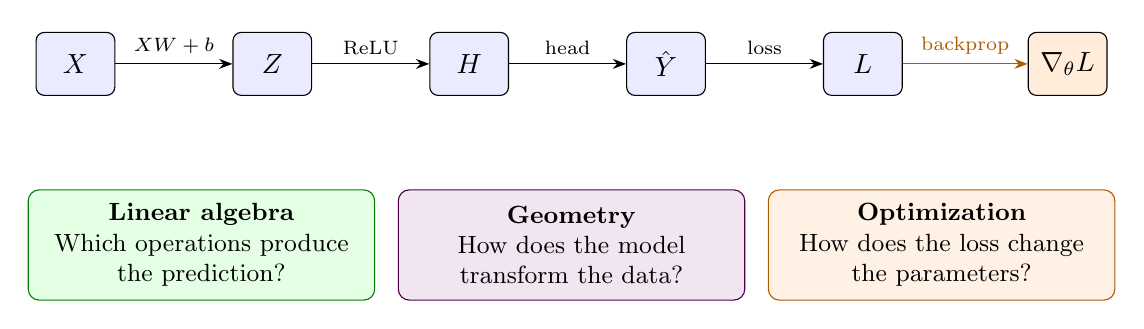
\begin{tikzpicture}[>=Stealth,
  nd/.style={draw,rounded corners=3pt,fill=blue!8,minimum width=10mm,minimum height=8mm},
  view/.style={draw,rounded corners=4pt,minimum width=4.4cm,minimum height=1.4cm,align=center,font=\small}]
\node[nd] (X) at (0,0) {$X$};
\node[nd] (Z) at (2.5,0) {$Z$};
\node[nd] (H) at (5,0) {$H$};
\node[nd] (Y) at (7.5,0) {$\hat Y$};
\node[nd] (L) at (10,0) {$L$};
\node[nd,fill=orange!15] (G) at (12.6,0) {$\nabla_\theta L$};
\draw[->] (X)--node[above,font=\scriptsize]{$XW+b$}(Z);
\draw[->] (Z)--node[above,font=\scriptsize]{ReLU}(H);
\draw[->] (H)--node[above,font=\scriptsize]{head}(Y);
\draw[->] (Y)--node[above,font=\scriptsize]{loss}(L);
\draw[->,orange!70!black] (L)--node[above,font=\scriptsize]{backprop}(G);
\node[view,fill=green!10,draw=green!50!black] at (1.6,-2.3) {\textbf{Linear algebra}\\Which operations produce\\the prediction?};
\node[view,fill=violet!10,draw=violet!60!black] at (6.3,-2.3) {\textbf{Geometry}\\How does the model\\transform the data?};
\node[view,fill=orange!10,draw=orange!70!black] at (11,-2.3) {\textbf{Optimization}\\How does the loss change\\the parameters?};
\end{tikzpicture}
\caption{Redrawn from slide 5: one forward--backward step and the three questions attached to it.}
\end{figure}

\begin{definition}[Forward step of an affine layer with ReLU]
Given a mini-batch $X\in\R^{B\times D}$, weights $W\in\R^{D\times H}$ and bias $b\in\R^{H}$, define
\[
Z = XW + \mathbf 1 b\T \in \R^{B\times H},\qquad H = \ReLU(Z)\ (\text{entrywise}),
\]
followed by a prediction $\hat Y$ and a scalar loss $L(\hat Y, Y)$. The gradient $\nabla_\theta L$ collects the derivatives of $L$ with respect to all parameters $\theta$ (here $W,b$ and the parameters of the head).
\end{definition}

\begin{intuition}
It is the same object seen through three lenses, like a car seen as a machine (linear algebra: which parts move), as a vehicle in space (geometry: where does it take the data) and as a driver receiving feedback (optimization: how to steer after a mistake). Each lens asks a different question, but all three are answered with the same matrix calculus.
\end{intuition}

\subsection{Fundamental mathematical disciplines for neural networks \slides{6}}

\begin{itemize}
  \item \textbf{Linear algebra}: vectors, matrices and tensors carry all computations; factorizations such as the SVD and the eigendecomposition support dimensionality reduction.
  \item \textbf{Geometry}: networks act in high-dimensional spaces; manifolds, distance metrics and transformations improve robustness and interpretability.
  \item \textbf{Optimization}: training is a large-scale optimization problem; gradient descent, Hessians and loss analysis make it effective.
\end{itemize}

\subsection{Two spaces that must not be confused \slides{7}}

\begin{definition}[Representation space and parameter space]
The \emph{representation space} is where examples and activations live: $X\mapsto Z=f_\theta(X)$, with $\theta$ fixed. The \emph{parameter space} is where models live: $\theta\mapsto L(\theta)$, with the data fixed.
\end{definition}

\begin{figure}[ht]
\centering
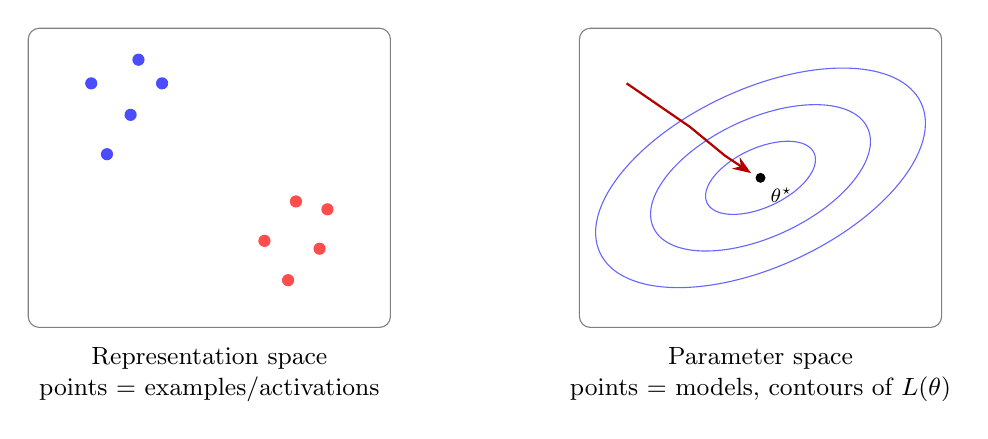
\begin{tikzpicture}[>=Stealth]
\begin{scope}
  \draw[rounded corners,gray] (-2.3,-1.9) rectangle (2.3,1.9);
  \foreach \x/\y in {-1.5/1.2,-1.0/0.8,-1.3/0.3,-0.6/1.2,-0.9/1.5} \fill[blue!70] (\x,\y) circle (2.2pt);
  \foreach \x/\y in {1.4/-0.9,1.0/-1.3,1.5/-0.4,0.7/-0.8,1.1/-0.3} \fill[red!70] (\x,\y) circle (2.2pt);
  \node[align=center,font=\small] at (0,-2.5) {Representation space\\points = examples/activations};
\end{scope}
\begin{scope}[xshift=7cm]
  \draw[rounded corners,gray] (-2.3,-1.9) rectangle (2.3,1.9);
  \begin{scope}[rotate=25]
    \foreach \r in {0.5,1,1.5} \draw[blue!60] (0,0) ellipse ({1.5*\r} and {0.75*\r});
  \end{scope}
  \draw[->,thick,red!70!black] (-1.7,1.2)--(-0.9,0.65)--(-0.45,0.28)--(-0.12,0.06);
  \fill (0,0) circle (1.8pt) node[below right,font=\scriptsize]{$\theta^\star$};
  \node[align=center,font=\small] at (0,-2.5) {Parameter space\\points = models, contours of $L(\theta)$};
\end{scope}
\end{tikzpicture}
\caption{Left: distances and directions between activations describe learned features. Right: gradients and curvature of $L(\theta)$ describe training dynamics.}
\end{figure}

\begin{intuition}
A neuron's activation is one coordinate of a point in the left picture, whereas its weight is one coordinate of a point in the right picture. For a dense layer $784\to128$, a batch of activations lives in $\R^{128}$ per example, but a \emph{single model} is a point in a space with $784\cdot128+128 = 100\,480$ dimensions. Same matrix calculus, completely different questions.
\end{intuition}

\subsection{Example: geometry of feature spaces \slides{8}}

An image classifier learns to map raw inputs to a representation where classes occupy distinct regions: similar examples cluster and different classes are well separated, so that a simple decision rule on the last layer suffices.

\begin{figure}[ht]
\centering
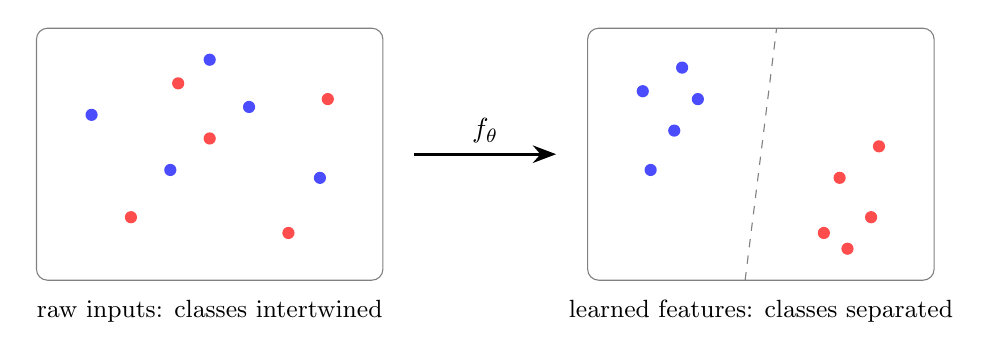
\begin{tikzpicture}[>=Stealth]
\begin{scope}
  \draw[rounded corners,gray] (-2.2,-1.6) rectangle (2.2,1.6);
  \foreach \x/\y in {-1.5/0.5,-0.5/-0.2,0.5/0.6,1.4/-0.3,0/1.2} \fill[blue!70] (\x,\y) circle (2.2pt);
  \foreach \x/\y in {-1.0/-0.8,0/0.2,1.0/-1.0,-0.4/0.9,1.5/0.7} \fill[red!70] (\x,\y) circle (2.2pt);
  \node[font=\small] at (0,-2.0) {raw inputs: classes intertwined};
\end{scope}
\draw[->,very thick] (2.6,0)--node[above]{$f_\theta$}(4.4,0);
\begin{scope}[xshift=7cm]
  \draw[rounded corners,gray] (-2.2,-1.6) rectangle (2.2,1.6);
  \foreach \x/\y in {-1.5/0.8,-1.1/0.3,-1.4/-0.2,-0.8/0.7,-1.0/1.1} \fill[blue!70] (\x,\y) circle (2.2pt);
  \foreach \x/\y in {1.4/-0.8,1.0/-0.3,1.5/0.1,0.8/-1.0,1.1/-1.2} \fill[red!70] (\x,\y) circle (2.2pt);
  \draw[dashed,gray] (-0.2,-1.6)--(0.2,1.6);
  \node[font=\small] at (0,-2.0) {learned features: classes separated};
\end{scope}
\end{tikzpicture}
\caption{Original figure for slide 8 (described only in prose there): the network turns an entangled input space into a feature space where a linear boundary works.}
\end{figure}

\subsection{Neural network as a composition of functions \slides{9--10}}

\begin{definition}[Feed-forward network as a composition]\label{def:comp}
With weight matrices $W_i$ (linear maps), bias vectors $b_i$ (shifts) and an activation $\sigma$ applied entrywise,
\begin{equation}\label{eq:comp}
f_\theta(X)=W_L\,\sigma\!\big(W_{L-1}\cdots\sigma(W_1X+b_1)\cdots+b_{L-1}\big)+b_L .
\end{equation}
\end{definition}

\begin{remark}[Column versus row convention]
Equation~\eqref{eq:comp} multiplies $X$ on the \emph{left} by $W_1$ (data as columns, $W_1\in\R^{D_{\rm out}\times D_{\rm in}}$), whereas the running example on slide~26 writes $Z=XW+b$ (data as rows, $W\in\R^{D_{\rm in}\times D_{\rm out}}$). The two are related by transposition, $(W_1X)\T = X\T W_1\T$. Always check which convention a formula or library uses.
\end{remark}

\begin{figure}[ht]
\centering
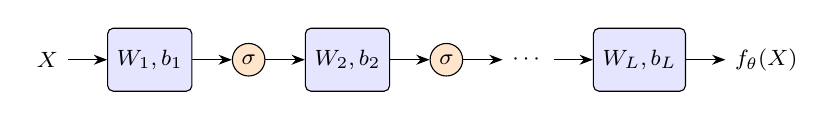
\begin{tikzpicture}[>=Stealth,font=\footnotesize,
  lin/.style={draw,rounded corners=2pt,fill=blue!10,minimum height=8mm,align=center},
  act/.style={draw,circle,fill=orange!20,inner sep=2pt}]
\node (x) {$X$};
\node[lin,right=5mm of x] (a1) {$W_1,b_1$};
\node[act,right=5mm of a1] (s1) {$\sigma$};
\node[lin,right=5mm of s1] (a2) {$W_2,b_2$};
\node[act,right=5mm of a2] (s2) {$\sigma$};
\node[right=5mm of s2] (d) {$\cdots$};
\node[lin,right=5mm of d] (aL) {$W_L,b_L$};
\node[right=5mm of aL] (y) {$f_\theta(X)$};
\foreach \a/\b in {x/a1,a1/s1,s1/a2,a2/s2,s2/d,d/aL,aL/y} \draw[->] (\a)--(\b);
\end{tikzpicture}
\caption{Equation~\eqref{eq:comp} as a chain: alternating affine maps (linear algebra) and pointwise nonlinearities.}
\end{figure}

The components of~\eqref{eq:comp} are: \emph{linear algebra} (matrix products such as $WX$ govern propagation), \emph{nonlinearity} ($\sigma(WX)$ makes the network expressive) and \emph{optimization} (minimizing a loss with gradient methods, e.g.\ $\nabla_W L$).

\textbf{Central question of the course.} What properties of the individual maps survive, grow or disappear under composition? This returns for expressivity, stability, gradients, recurrence and depth.

\begin{proposition}[Without nonlinearity, depth collapses]\label{prop:collapse}
If $\sigma=\mathrm{id}$, then $f_\theta$ in~\eqref{eq:comp} is a single affine map $X\mapsto \widetilde W X+\tilde b$.
\end{proposition}
\begin{proof}
For $L=2$: $W_2(W_1X+b_1)+b_2=(W_2W_1)X+(W_2b_1+b_2)$. Induction on $L$: the composition of two affine maps is affine, since $W'(WX+b)+b'=(W'W)X+(W'b+b')$.
\end{proof}

\begin{intuition}
Stacking linear layers is like doing several successive currency conversions: however many you chain, the result is one exchange rate plus a fixed fee. Only the nonlinearity $\sigma$ lets extra layers add something new. Numerically, $W_1=\begin{bmatrix}1&2\end{bmatrix}^{\!\top}$ (a $2\times1$ map), $W_2=\begin{bmatrix}3&-1\end{bmatrix}$ compose to $W_2W_1=3\cdot1+(-1)\cdot 2=1$: two layers, one number.
\end{intuition}

%====================================================================
\section{Linear Algebra for Neural Networks \slides{11--26}}
%====================================================================

\subsection{Introduction to Linear Algebra \slides{11--13}}

Fluency with vectors and matrices --- multiplication, transposition, inverses --- is essential for neural networks, and it is what makes backpropagation and optimization approachable. It is best learned by consistent practice; Python libraries (NumPy, PyTorch) make the operations directly executable.

\textbf{Advantages of linear algebra} (slide 12): compact notation; an intuitive geometric picture (transformations, feature spaces); a convenient set of operations (decompositions, optimizations); data structures suited to images, text and sequences; a universal language in the literature; and an easy equation-to-code translation.

\begin{figure}[ht]
\centering
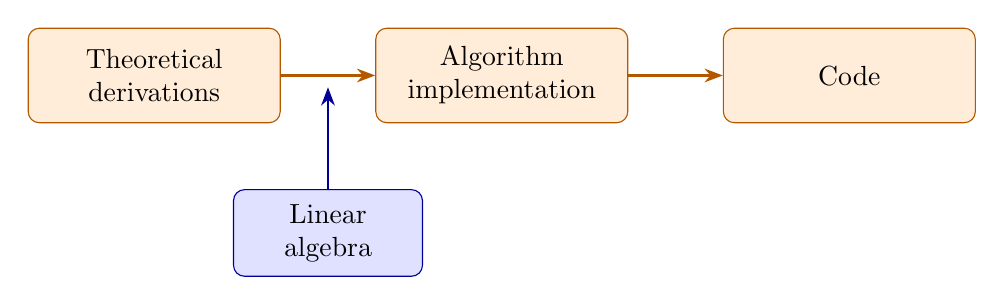
\begin{tikzpicture}[>=Stealth,
  blk/.style={draw=orange!70!black,fill=orange!15,rounded corners=4pt,minimum width=3.2cm,minimum height=1.2cm,align=center}]
\node[blk] (a) {Theoretical\\derivations};
\node[blk,right=1.2cm of a] (b) {Algorithm\\implementation};
\node[blk,right=1.2cm of b] (c) {Code};
\draw[->,thick,orange!70!black] (a)--(b);
\draw[->,thick,orange!70!black] (b)--(c);
\node[draw=blue!60!black,fill=blue!12,rounded corners=4pt,minimum width=2.4cm,minimum height=1.1cm,align=center]
  (la) at ($(a.east)!0.5!(b.west)+(0,-2.0)$) {Linear\\algebra};
\draw[->,thick,blue!60!black] (la.north)--($(a.east)!0.5!(b.west)+(0,-0.15)$);
\end{tikzpicture}
\caption{Redrawn from Figure 1 of the slides: linear algebra is the glue that turns theory into an algorithm whose form maps directly to code.}
\end{figure}

\begin{intuition}
Compare $y_i=\sum_j W_{ij}x_j+b_i$ written for each $i$ with $y=Wx+b$: the second line is both the mathematical statement and (almost character by character) the NumPy line \texttt{y = W @ x + b}. That is the ``equation-to-code'' advantage.
\end{intuition}

\subsection{Algebraic Structures for Neural Networks \slides{14--24}}

Neural networks process data as numerical structures: \emph{scalar} $x\in\R$, \emph{vector} $\mathbf x\in\R^n$, \emph{matrix} $\mathbf X\in\R^{M\times N}$ and \emph{tensor} $\mathcal X\in\R^{d_1\times\cdots\times d_n}$. Each encodes a different kind of information.

\paragraph{Scalars \slides{15}.} A scalar is a single real number (lowercase letter, $x\in\R$), e.g.\ the amplitude of a signal sample, one pixel value, or the numerical value of a single neuron.

\paragraph{Vectors \slides{16--17}.}
\begin{definition}[Vector]
A vector is an ordered arrangement of scalars, denoted by a bold lowercase letter, $\mathbf x\in\R^n$, e.g.\ $\mathbf x=[1,\,0.3,\,-2]$. Geometrically it is the path from the origin to a point $P$ in an $N$-dimensional space.
\end{definition}

\begin{figure}[ht]
\centering
\begin{tikzpicture}[>=Stealth]
\draw[->,thick] (0,0)--(0,3.4) node[above]{$z$};
\draw[->,thick] (0,0)--(4.4,0) node[right]{$y$};
\draw[->,thick] (0,0)--(-1.6,-1.4) node[below left]{$x$};
\draw[->,very thick,red!50!black] (0,0)--(1.6,2.7);
\draw[->,very thick,teal] (0,0)--(3.6,0.9);
\fill (1.6,2.7) circle (1.5pt) node[right,font=\scriptsize]{$P_1(x_1,y_1,z_1)$};
\fill (3.6,0.9) circle (1.5pt) node[above right,font=\scriptsize]{$P_2(x_2,y_2,z_2)$};
\end{tikzpicture}
\caption{Redrawn from Figure 2 of the slides: vectors as arrows from the origin to points.}
\end{figure}

As input data, a vector represents a 1D digital signal (audio, brain signal, time series): an ordered sequence of samples, stored by convention as a \emph{column} vector. (The slide writes $\mathbf x=[x_1\ x_2\ x_3]$ as a row for typographic economy, but states the column convention; I use columns and write $\mathbf x\T$ for rows.) In networks, a vector may represent a layer or a sequence of weights.

\paragraph{Matrices \slides{18--21}.}
\begin{definition}[Matrix]
A matrix $\mathbf X\in\R^{M\times N}$ is an array with $M$ rows and $N$ columns, $\mathbf X=[\mathbf x_1\ \cdots\ \mathbf x_N]=(x_{ij})$. It can be seen as a vertical stack of row vectors or a horizontal arrangement of column vectors.
\end{definition}

As input data, matrices represent 2D signals (grayscale images) or collections of 1D signals (multichannel audio, multisensor recordings); in networks, they store weights.

\begin{example}[Data, weights, activations \slides{20--21}]
A grayscale image is a matrix of pixel intensities; a colour image is a tensor of shape (height, width, 3). A dataset of $m$ samples with $n$ features is $\mathbf X\in\R^{m\times n}$ (one row per sample, one column per feature). A layer with input $\mathbf x\in\R^n$ and weights $\mathbf W\in\R^{m\times n}$ outputs $\mathbf y=\mathbf W\mathbf x+\mathbf b$. For instance, with $n=3$, $m=2$,
\[
\mathbf W=\begin{bmatrix}1&0&2\\-1&1&0\end{bmatrix},\ 
\mathbf x=\begin{bmatrix}1\\2\\3\end{bmatrix},\ 
\mathbf b=\begin{bmatrix}0\\1\end{bmatrix}
\ \Rightarrow\ 
\mathbf y=\begin{bmatrix}7\\1\end{bmatrix}+\begin{bmatrix}0\\1\end{bmatrix}=\begin{bmatrix}7\\2\end{bmatrix}.
\]
\end{example}

\paragraph{Tensors \slides{22--24}.}
\begin{definition}[Tensor]
A tensor $\mathcal X\in\R^{d_1\times d_2\times\cdots\times d_n}$ is a function of three or more indices; equivalently a stacking of $K$ matrices (slices), $\mathcal X=\{\mathbf X_1,\dots,\mathbf X_K\}$, or of higher-order tensors along horizontal, vertical or lateral slices. It generalizes the matrix.
\end{definition}

Tensors represent 3D signals (video, time-frequency maps of EEG) and higher-dimensional data (MR brain imaging).

\begin{figure}[ht]
\centering
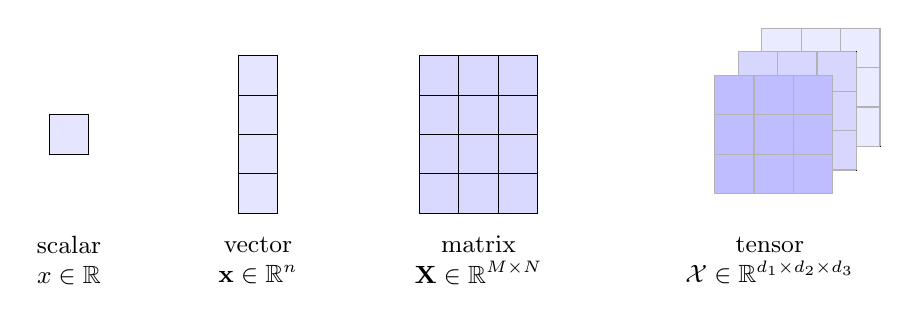
\begin{tikzpicture}[cell/.style={draw,minimum size=5mm,inner sep=0pt,fill=blue!10}, lab/.style={font=\small,align=center}]
\node[cell] at (0,0) {};
\node[lab] at (0,-1.6) {scalar\\$x\in\R$};
\foreach \i in {0,1,2,3} \node[cell] at (2.4,0.75-0.5*\i) {};
\node[lab] at (2.4,-1.6) {vector\\$\mathbf x\in\R^{n}$};
\foreach \i in {0,1,2,3} \foreach \j in {0,1,2} \node[cell,fill=blue!15] at (4.7+0.5*\j,0.75-0.5*\i) {};
\node[lab] at (5.2,-1.6) {matrix\\$\mathbf X\in\R^{M\times N}$};
\foreach \k/\c in {2/blue!8,1/blue!16,0/blue!26} {
  \draw[fill=\c] (8.2+0.3*\k,-0.75+0.3*\k) rectangle ++(1.5,1.5);
  \draw[step=0.5cm,gray!60,shift={(8.2+0.3*\k,-0.75+0.3*\k)}] (0,0) grid (1.5,1.5);
}
\node[lab] at (8.9,-1.6) {tensor\\$\mathcal X\in\R^{d_1\times d_2\times d_3}$};
\end{tikzpicture}
\caption{Original figure: scalar $\subset$ vector $\subset$ matrix $\subset$ tensor as increasing numbers of indices (0, 1, 2, 3).}
\end{figure}

\begin{figure}[ht]
\centering
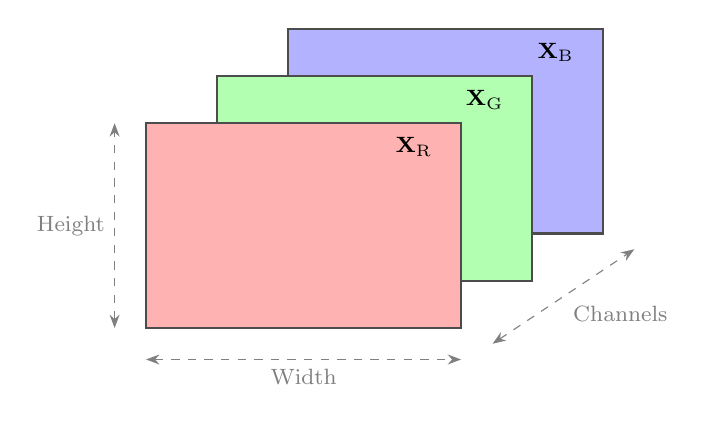
\begin{tikzpicture}[>=Stealth]
\foreach \k/\c/\n in {2/blue!30/B,1/green!30/G,0/red!30/R} {
  \draw[fill=\c,draw=black!70,thick] (0.9*\k,0.6*\k) rectangle ++(4,2.6);
  \node[font=\footnotesize] at (0.9*\k+3.4,0.6*\k+2.3) {$\mathbf X_{\mathrm{\n}}$};
}
\draw[<->,dashed,gray] (-0.4,0)--(-0.4,2.6) node[midway,left,font=\footnotesize]{Height};
\draw[<->,dashed,gray] (0,-0.4)--(4,-0.4) node[midway,below,font=\footnotesize]{Width};
\draw[<->,dashed,gray] (4.4,-0.2)--(6.2,1.0) node[midway,below right,font=\footnotesize]{Channels};
\end{tikzpicture}
\caption{Redrawn from Figure 6 of the slides: a colour image as a 3D tensor $\mathcal X=\{\mathbf X_R,\mathbf X_G,\mathbf X_B\}$ of three channel matrices. (The slide labels the horizontal axis ``Weight''; it is the image \emph{width}.)}
\end{figure}

\begin{intuition}
Order of the tensor = number of indices needed to locate one scalar. A $224\times224$ RGB image needs three indices and holds $3\cdot224\cdot224=150\,528$ numbers; a batch of $32$ such images needs four indices and holds $4\,816\,896$ numbers. Nothing new happens mathematically --- there are just more indices to keep track of.
\end{intuition}

\subsection{Data Shapes \slides{25--26}}

\begin{definition}[Semantics of axes \slides{25}]
The \emph{shape} of a tensor is the tuple of its axis lengths. Its meaning comes from the \emph{labels} of the axes, not from its order:
\begin{center}
\small
\begin{tabular}{@{}lll@{}}
\toprule
Object & Typical shape & Meaning\\\midrule
Tabular batch & $B\times D$ & examples $\times$ features\\
Image batch & $B\times C\times H\times W$ & examples $\times$ channels $\times$ space\\
Token batch & $B\times T\times D$ & examples $\times$ tokens $\times$ features\\
Dense weights & $D_{\rm out}\times D_{\rm in}$ & output $\times$ input features\\\bottomrule
\end{tabular}
\end{center}
\end{definition}

\begin{intuition}
A tensor of shape $32\times64\times64$ could be 32 grayscale images, 32 sequences of 64 tokens with 64 features each, or something else entirely. Only the axis labels tell you which, and shapes will be central for CNN layouts, sequence models and multi-head attention.
\end{intuition}

\begin{example}[Running example: one mini-batch \slides{26}]\label{ex:running}
Let $X\in\R^{3\times2}$, $W\in\R^{2\times4}$, $b\in\R^{4}$. The affine layer acts on every row: $Z=XW+\mathbf 1b\T\in\R^{3\times4}$ (broadcasting: the same bias is added to all three examples). With
\[
X=\begin{bmatrix}1&2\\0&-1\\3&1\end{bmatrix},\quad
W=\begin{bmatrix}1&0&-1&2\\2&1&0&-1\end{bmatrix},\quad
b=\begin{bmatrix}0.5&-1&0&1\end{bmatrix}
\]
we get
\[
XW=\begin{bmatrix}5&2&-1&0\\-2&-1&0&1\\5&1&-3&5\end{bmatrix},\qquad
Z=\begin{bmatrix}5.5&1&-1&1\\-1.5&-2&0&2\\5.5&0&-3&6\end{bmatrix},\qquad
\ReLU(Z)=\begin{bmatrix}5.5&1&0&1\\0&0&0&2\\5.5&0&0&6\end{bmatrix}.
\]
E.g.\ $Z_{11}=1\cdot1+2\cdot2+0.5=5.5$.
\end{example}

\begin{algorithm}[Shape checking]\label{alg:shape}
To verify a matrix expression before running any code: (1) write the shape of every operand with labelled axes; (2) for each product $(N\times P)(P\times M)$ check that the inner sizes agree; (3) the result has shape $N\times M$ and the shared axis has been \emph{contracted}; (4) for a sum, check the shapes are equal or broadcastable (bias: $B\times H$ plus $H$).
\end{algorithm}

\begin{intuition}
Shape checking is dimensional analysis for tensors: like verifying that both sides of a physics formula are in metres, it catches many implementation errors before any data is processed. In Example~\ref{ex:running}: $(3\times2)(2\times4)\to3\times4$, the axis of size~2 is contracted, and $b$ (length 4) is broadcast over the 3 rows.
\end{intuition}

%====================================================================
\section{Data Manipulation with Algebraic Operations \slides{27--54}}
%====================================================================

\subsection{Simple Algebraic Operations on Data \slides{27--31}}

\paragraph{Basic operations on vectors \slides{27}.} For $\mathbf a,\mathbf b\in\R^n$ and $\lambda\in\R$: addition $c_i=a_i+b_i$; scalar multiplication $(\lambda\mathbf a)_i=\lambda a_i$; and the dot product $\mathbf a\cdot\mathbf b=\sum_{i=1}^n a_ib_i$, which measures the similarity of two vectors.

\paragraph{How algebraic operations affect data \slides{28--29}.} Feature weighting (dot products compute the weighted sums in neurons); feature scaling (multiply each feature by a constant); feature transformation (linear maps into new feature spaces); data centering (subtract the mean); dimensionality reduction (PCA via matrix decompositions); covariance computation (matrix products); convolution (linear combinations of shifted inputs, highlighting edges, textures and shapes); and data augmentation (rotation and scaling matrices).

\begin{algorithm}[Centering and covariance of a data matrix]\label{alg:cov}
Given $X\in\R^{m\times n}$ (rows = samples): (1) $\mu=\tfrac1m X\T\mathbf 1\in\R^n$; (2) $X_c=X-\mathbf 1\mu\T$; (3) $C=\tfrac1{m-1}X_c\T X_c\in\R^{n\times n}$.
\end{algorithm}

\begin{example}
Take $X=\begin{bmatrix}1&2\\3&4\\5&9\end{bmatrix}$. Then $\mu=[3,5]\T$, $X_c=\begin{bmatrix}-2&-3\\0&-1\\2&4\end{bmatrix}$ and
$X_c\T X_c=\begin{bmatrix}8&14\\14&26\end{bmatrix}$, so $C=\begin{bmatrix}4&7\\7&13\end{bmatrix}$ (feature 1 has variance 4, feature 2 has variance 13, covariance 7).
\end{example}

\begin{intuition}
Centering moves the data cloud so that its centre of mass sits at the origin; the covariance matrix then records, entry by entry, how strongly two features move together. Both steps are just a subtraction and one matrix product --- which is why they are cheap and why PCA (next lectures) can be phrased entirely in linear algebra.
\end{intuition}

\paragraph{Additions and multiplications with matrices \slides{30}.}
\begin{definition}[Matrix sum and product]
For $A,B\in(\R,\C)^{N\times M}$, $C=A+B$ has entries $c_{ij}=a_{ij}+b_{ij}$. For $A\in(\R,\C)^{N\times P}$, $B\in(\R,\C)^{P\times M}$, $C=AB\in(\R,\C)^{N\times M}$ has
\[
c_{ij}=\sum_{k=1}^{P}a_{ik}b_{kj}.
\]
\end{definition}

The product costs $N\cdot P\cdot M$ scalar multiplications; e.g.\ $(32\times128)(128\times64)$ needs $32\cdot128\cdot64=262\,144$.

\paragraph{Addition and multiplication in general algebraic structures \slides{31}.}
\begin{definition}[Group, ring, field]
A \emph{group} $(G,+)$ is a set with an operation that is closed, associative, has an identity and inverses. A \emph{ring} $(R,+,\cdot)$ is an abelian group under $+$ with an associative product that distributes over $+$. A \emph{field} is a (commutative) ring in which every nonzero element has a multiplicative inverse.
\end{definition}

\begin{example}
$\R$ is a field: addition and multiplication are closed and associative, every number has an additive inverse, and every nonzero number has a multiplicative inverse. The set $\R^{n\times n}$ is a ring but \emph{not} a field: with $A=\begin{bmatrix}1&1\\0&1\end{bmatrix}$, $B=\begin{bmatrix}1&0\\1&1\end{bmatrix}$, $AB=\begin{bmatrix}2&1\\1&1\end{bmatrix}\neq\begin{bmatrix}1&1\\1&2\end{bmatrix}=BA$, and $N=\begin{bmatrix}0&1\\0&0\end{bmatrix}\ne0$ satisfies $N^2=0$.
\end{example}

\begin{intuition}
Numbers behave so nicely that we forget they are special: one can divide, order does not matter. Matrices give up commutativity and general division, and this is exactly why the \emph{order} of layers matters and why Sections~\ref{sec:inv}--3.6 on inverses and rank are needed. (Floating-point numbers only approximate a field --- rounding errors are the other side of ``stable computations''.)
\end{intuition}

\subsection{Inner and Outer Products \slides{32--33}}

\begin{definition}[Inner and outer product]
For $\mathbf u,\mathbf v\in(\R,\C)^{N}$ the inner (scalar, dot) product is
\[
\langle\mathbf u,\mathbf v\rangle=\mathbf v\Her\mathbf u=\sum_{i=1}^{N}u_iv_i^{*}.
\]
For $\mathbf u\in(\R,\C)^{M}$, $\mathbf v\in(\R,\C)^{N}$ the outer product is the matrix
\[
\mathbf u\mathbf v\Her=\begin{bmatrix}u_1v_1^*&\cdots&u_1v_N^*\\\vdots&\ddots&\vdots\\u_Mv_1^*&\cdots&u_Mv_N^*\end{bmatrix}\in(\R,\C)^{M\times N}.
\]
\end{definition}

\begin{remark}
The slide's typeset chain of equalities for $\langle\mathbf u,\mathbf v\rangle$ is garbled in the PDF; the final sum $\sum u_iv_i^*$ is what I use, which equals $\mathbf v\Her\mathbf u$. (The other convention $\mathbf u\Her\mathbf v=\sum u_i^*v_i$ is its complex conjugate.) In the real case all conventions coincide.
\end{remark}

\begin{proposition}
For real vectors the inner product is bilinear and symmetric, and $\langle\mathbf u,\mathbf u\rangle=\sum u_i^2\ge0$ with equality iff $\mathbf u=0$. The outer product $\mathbf u\mathbf v\T$ has rank at most one, and $(\mathbf u\mathbf v\T)_{ij}=u_iv_j$.
\end{proposition}
\begin{proof}
Bilinearity and symmetry follow from the definition of the sum. Positivity: a sum of squares vanishes iff every term does. Every column of $\mathbf u\mathbf v\T$ is a multiple ($v_j$) of $\mathbf u$, so its column space is spanned by $\mathbf u$.
\end{proof}

\begin{intuition}
The dot product multiplies matching coordinates and adds them up: large and positive when the two vectors point the same way, zero when they are orthogonal, negative when they oppose. This is exactly what a neuron does when it weighs an input against its weights. The outer product does the opposite of collapsing: from $\mathbf u=[1,2]\T$, $\mathbf v=[3,0,1]\T$ it builds the whole table $\begin{bmatrix}3&0&1\\6&0&2\end{bmatrix}$ of pairwise products, a rank-one matrix. Outer products will reappear as the gradient of a linear layer.
\end{intuition}

\paragraph{Matrix multiplication is a contraction \slides{33}.}
\begin{definition}[Contraction]
For $X\in\R^{B\times D}$ and $W\in\R^{D\times H}$,
\[
Z_{bh}=\sum_{d=1}^{D}X_{bd}W_{dh}.
\]
The index $d$ disappears because it is summed over (\emph{contracted}); $b$ and $h$ remain. Rule: a \emph{repeated} index is contracted, an \emph{unrepeated} index appears in the output.
\end{definition}

\begin{figure}[ht]
\centering
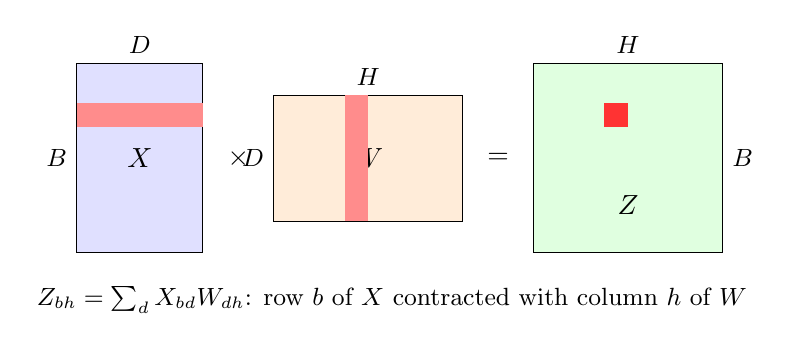
\begin{tikzpicture}[lab/.style={font=\small}]
\draw[fill=blue!12] (0,0) rectangle (1.6,2.4); \node at (0.8,1.2) {$X$};
\node[lab,above] at (0.8,2.4) {$D$}; \node[lab,left] at (0,1.2) {$B$};
\node at (2.05,1.2) {$\times$};
\draw[fill=orange!15] (2.5,0.4) rectangle (4.9,2.0); \node at (3.7,1.2) {$W$};
\node[lab,above] at (3.7,2.0) {$H$}; \node[lab,left] at (2.5,1.2) {$D$};
\node at (5.35,1.2) {$=$};
\draw[fill=green!12] (5.8,0) rectangle (8.2,2.4); \node at (7.0,0.6) {$Z$};
\node[lab,above] at (7.0,2.4) {$H$}; \node[lab,right] at (8.2,1.2) {$B$};
\fill[red!45] (0,1.6) rectangle (1.6,1.9);
\fill[red!45] (3.4,0.4) rectangle (3.7,2.0);
\fill[red!80] (6.7,1.6) rectangle (7.0,1.9);
\node[lab] at (4,-0.6) {$Z_{bh}=\sum_d X_{bd}W_{dh}$: row $b$ of $X$ contracted with column $h$ of $W$};
\end{tikzpicture}
\caption{Original figure: matrix product as a contraction of the shared axis $D$. The red row and column combine into one red entry.}
\end{figure}

\begin{intuition}
Reading an equation by its indices is faster than reading it by its symbols: any repeated index is ``used up'', anything left over is the shape of the result. The same viewpoint carries unchanged from dense layers to attention and tensor networks.
\end{intuition}

\subsection{Dealing with Matrices \slides{34--44}}

\paragraph{Hadamard product \slides{34--36}.}
\begin{definition}[Hadamard product]
For $A,B\in\R^{N\times M}$, $(A\Had B)_{ij}=a_{ij}b_{ij}$.
\end{definition}

Unlike the matrix product it does not sum over shared indices; it is used for elementwise transformations, feature-wise scaling, attention mechanisms, weighting features in activations and elementwise normalization.

\begin{proposition}\label{prop:hadamard}
The Hadamard product is commutative, associative and distributes over $+$. If $D_{\mathbf a}=\diag(\mathbf a)$ then $D_{\mathbf a}\mathbf x=\mathbf a\Had\mathbf x$ and $D_{\mathbf a}D_{\mathbf b}=D_{\mathbf a\Had\mathbf b}$.
\end{proposition}
\begin{proof}
All three algebraic laws are inherited entry by entry from multiplication of real numbers. For the diagonal statement, $(D_{\mathbf a}\mathbf x)_i=\sum_k(D_{\mathbf a})_{ik}x_k=a_ix_i$, and $(D_{\mathbf a}D_{\mathbf b})_{ij}=a_i\delta_{ij}b_j=a_ib_i\delta_{ij}$.
\end{proof}

\begin{figure}[ht]
\centering
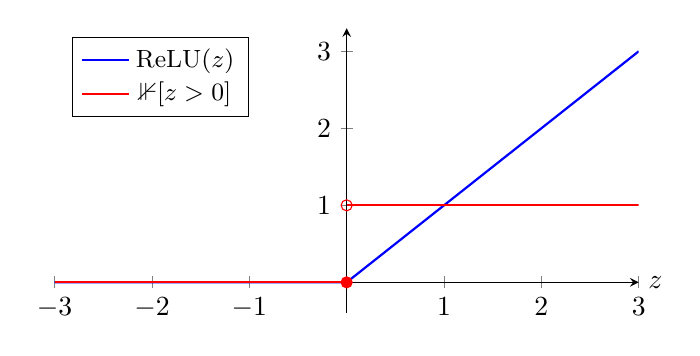
\begin{tikzpicture}
\begin{axis}[width=9cm,height=5.2cm,axis lines=middle,xlabel={$z$},xmin=-3,xmax=3,ymin=-0.4,ymax=3.3,
  legend pos=north west,legend style={font=\small},xlabel style={at={(ticklabel* cs:1)},anchor=west}]
\addplot[thick,blue] coordinates {(-3,0)(0,0)(3,3)}; \addlegendentry{$\ReLU(z)$}
\addplot[thick,red] coordinates {(-3,0)(0,0)}; \addlegendentry{$\ind{z>0}$}
\addplot[thick,red,forget plot] coordinates {(0,1)(3,1)};
\addplot[only marks,mark=*,red,forget plot] coordinates {(0,0)};
\addplot[only marks,mark=o,red,forget plot] coordinates {(0,1)};
\end{axis}
\end{tikzpicture}
\caption{Original figure: $\ReLU$ and its derivative, the binary mask $\ind{z>0}$ (value $0$ at $z=0$ by convention).}
\end{figure}

\paragraph{Matrix product and Hadamard product answer different questions \slides{36}.}
The matrix product $Z=XW$ \emph{mixes} information across the contracted feature axis; the Hadamard product $H=G\Had Z$ applies an elementwise gate or mask, for which shapes must be compatible. For $\ReLU$ the backward pass contains the binary mask
\[
\frac{\partial\,\ReLU(Z)}{\partial Z}=\ind{Z>0}.
\]

\begin{intuition}
Matrix product = a meeting where every feature talks to every other one. Hadamard product = a switchboard where each entry is individually multiplied by its own dial. In Example~\ref{ex:running} the mask of $Z$ is $\begin{bmatrix}1&1&0&1\\0&0&0&1\\1&0&0&1\end{bmatrix}$: during backpropagation, gradient flows only through the entries marked $1$, i.e.\ $\partial L/\partial Z=\partial L/\partial H\Had\ind{Z>0}$. The same elementwise mechanism appears in LSTM gates, selective SSMs and attention masks.
\end{intuition}

\paragraph{Kronecker product \slides{37}.}
\begin{definition}[Kronecker product]
For $A\in(\R,\C)^{P\times Q}$ and $B\in(\R,\C)^{N\times M}$,
\[
A\otimes B=\begin{bmatrix}a_{11}B&\cdots&a_{1Q}B\\\vdots&\ddots&\vdots\\a_{P1}B&\cdots&a_{PQ}B\end{bmatrix}\in(\R,\C)^{PN\times QM}.
\]
\end{definition}

\begin{remark}
If $A$ and $B$ represent linear maps $T_1:X_1\to Y_1$ and $T_2:X_2\to Y_2$, then $A\otimes B$ represents the tensor product map $X_1\otimes X_2\to Y_1\otimes Y_2$.
\end{remark}

\begin{intuition}
The Kronecker product is ``a copy of $B$ scaled by each entry of $A$'', arranged as blocks. Sizes multiply: $(2\times2)\otimes(3\times3)$ is $6\times6$. For $A=\begin{bmatrix}1&2\\0&1\end{bmatrix}$, $B=\begin{bmatrix}1&1\end{bmatrix}$ the result is $\begin{bmatrix}1&1&2&2\\0&0&1&1\end{bmatrix}$. It is the matrix form of acting with two independent maps on two independent factors (e.g.\ rows and columns of an image); see the Appendix for the identity connecting it to $\vecop$.
\end{intuition}

\paragraph{Transpose matrix \slides{38--39}.}
\begin{definition}[Transpose]
For $A\in\R^{N\times M}$, $A\T\in\R^{M\times N}$ interchanges rows and columns: $(A\T)_{ij}=a_{ji}$. Hence $(A\T)\T=A$. Transposing a 2D signal swaps its two dimensions.
\end{definition}

\begin{remark}
On slide 38 the printed transpose shows the entry $a_{11}$ in position $(2,2)$ (``$a_{12}\ a_{11}\ \cdots$''); this is a typo for $a_{22}$.
\end{remark}

\paragraph{Hermitian matrix \slides{40}.}
\begin{definition}[Hermitian transpose]
For $A\in\K^{N\times M}$, $A\Her=(a_{ji}^*)$: transpose plus complex conjugation. In the real domain $A\Her=A\T$.
\end{definition}
Uses in the slides: Hermitian (self-adjoint) operators in quantum neural networks; kernels in SVMs and Gaussian processes; spectral decomposition of a Hermitian kernel matrix for dimensionality reduction.

\begin{proposition}[Transpose rules]\label{prop:transp}
$(AB)\Her=B\Her A\Her$, $(A+B)\Her=A\Her+B\Her$, and $(ABC\cdots)\Her=\cdots C\Her B\Her A\Her$.
\end{proposition}
\begin{proof}
$\big((AB)\Her\big)_{ij}=\big(\sum_k a_{jk}b_{ki}\big)^*=\sum_k b_{ki}^*a_{jk}^*=\sum_k (B\Her)_{ik}(A\Her)_{kj}$. The rule for sums is immediate; longer products follow by induction.
\end{proof}

\begin{intuition}
Transposing a product reverses the order --- like taking off socks and shoes, you undo the last step first. This reversal is exactly what makes gradients travel backwards through a network: $\partial L/\partial X=\partial L/\partial Z\;W\T$.
\end{intuition}

\paragraph{Matrices as row or column vectors \slides{41--42}.}
The $i$-th row of $A\in(\R,\C)^{N\times M}$ is $\mathbf a_i\in(\R,\C)^{1\times M}$ and its $j$-th column is $\mathbf a_j\in(\R,\C)^{N\times1}$; $A$ is a stack of $N$ rows or an arrangement of $M$ columns.

\begin{definition}[Vectorization]
$\vecop(A)\in(\R,\C)^{NM\times1}$ stacks the columns of $A$:
\[
\vecop(A)=[a_{11},\dots,a_{N1},\,a_{12},\dots,a_{N2},\,\dots,\,a_{1M},\dots,a_{NM}]\Her .
\]
\end{definition}

\begin{figure}[ht]
\centering
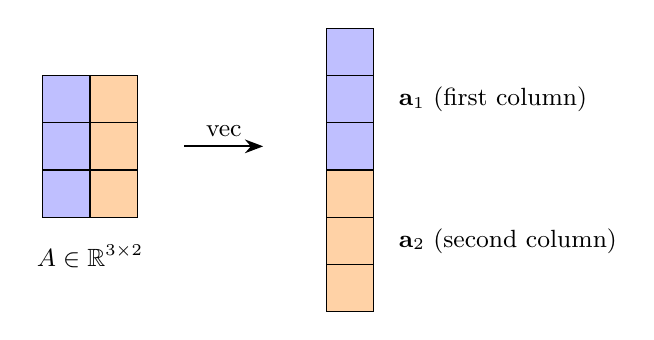
\begin{tikzpicture}[>=Stealth,
  c1/.style={draw,minimum size=6mm,inner sep=0,fill=blue!25},
  c2/.style={draw,minimum size=6mm,inner sep=0,fill=orange!35}]
\foreach \i in {0,1,2} {\node[c1] at (0,-0.6*\i) {}; \node[c2] at (0.6,-0.6*\i) {};}
\node[font=\small] at (0.3,-2.0) {$A\in\R^{3\times2}$};
\draw[->,thick] (1.5,-0.6)--(2.5,-0.6) node[midway,above,font=\small]{$\vecop$};
\foreach \i in {0,1,2} {\node[c1] at (3.6,0.6-0.6*\i) {}; \node[c2] at (3.6,-1.2-0.6*\i) {};}
\node[font=\small,anchor=west] at (4.1,0.0) {$\mathbf a_1$ (first column)};
\node[font=\small,anchor=west] at (4.1,-1.8) {$\mathbf a_2$ (second column)};
\end{tikzpicture}
\caption{Original figure: $\vecop$ stacks the columns of a $3\times2$ matrix into a $6\times1$ vector.}
\end{figure}

\paragraph{Transpose, reshape and permutation \slides{43}.} These operations can preserve values while changing how axes are interpreted:
\begin{center}
\small
\begin{tabular}{@{}lll@{}}
\toprule
Operation & What changes? & Typical use\\\midrule
$X\T$ & row/column order & dot products, covariance\\
reshape & grouping of axes & heads, patches, flattening\\
permute & axis order & channel-first vs channel-last\\\bottomrule
\end{tabular}
\end{center}
\textbf{Caution:} a legal reshape need not preserve the intended semantic correspondence between axes.

\begin{intuition}
Reshaping is like re-cutting a deck of cards into different piles: the cards (values) are unchanged, but which cards sit together, and therefore what a later operation combines, has changed. Reshaping a $6\times1$ vector to $2\times3$ and $3\times2$ gives different matrices; only one may be the one you meant.
\end{intuition}

\paragraph{Exercise: shape detective \slides{44}.} Let $X\in\R^{32\times128}$ and $W_Q,W_K\in\R^{128\times64}$. (1) Shapes of $Q=XW_Q$ and $K=XW_K$? (2) Shape of $QK\T$? (3) Which axis is contracted in each product?

\begin{example}[Solution]
(1) Both are $32\times64$. (2) $K\T$ is $64\times32$, so $QK\T\in\R^{32\times32}$. (3) In $XW_Q$ and $XW_K$ the axis of size $128$ (features) is contracted; in $QK\T$ the axis of size $64$ is contracted, leaving one score per pair of the 32 rows. Cost of $QK\T$: $32\cdot64\cdot32=65\,536$ multiplications.
\end{example}

\begin{figure}[ht]
\centering
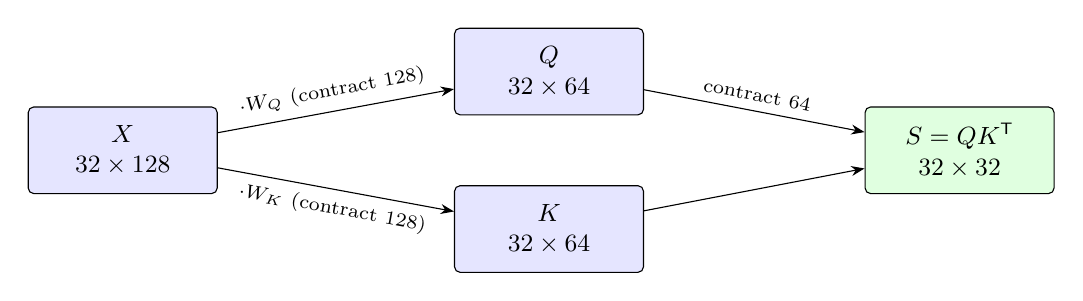
\begin{tikzpicture}[>=Stealth,shp/.style={draw,rounded corners=2pt,fill=blue!10,align=center,minimum width=2.4cm,minimum height=1.1cm,font=\small}]
\node[shp] (X) {$X$\\$32\times128$};
\node[shp,right=3cm of X,yshift=1cm] (Q) {$Q$\\$32\times64$};
\node[shp,right=3cm of X,yshift=-1cm] (K) {$K$\\$32\times64$};
\node[shp,fill=green!12,right=2.8cm of Q,yshift=-1cm] (S) {$S=QK\T$\\$32\times32$};
\draw[->] (X)--node[above,sloped,font=\scriptsize]{$\cdot W_Q$ (contract 128)}(Q);
\draw[->] (X)--node[below,sloped,font=\scriptsize]{$\cdot W_K$ (contract 128)}(K);
\draw[->] (Q)--node[above,sloped,font=\scriptsize]{contract 64}(S);
\draw[->] (K)--(S);
\end{tikzpicture}
\caption{Original figure: shape flow of the exercise, the core of self-attention scores.}
\end{figure}

\subsection{Special Matrices \slides{45--48}}

\paragraph{Diagonal matrix \slides{45}.}
$A\in(\R,\C)^{N\times N}$ is \emph{diagonal} if $a_{ij}=0$ for $i\ne j$. The operator $\diag$ builds a diagonal matrix from a vector, $A=\diag(\mathbf a)$, and extracts the diagonal, $\mathbf a=\diag^{-1}(A)$.

\paragraph{Trace and symmetry \slides{46}.}
\begin{definition}[Trace, symmetric, Hermitian]
$\tr(A)=\sum_{i=1}^Na_{ii}$. A matrix is \emph{symmetric} if $A\T=A$ (real) and \emph{Hermitian} if $A\Her=A$ (complex, $a_{ji}=a_{ij}^*$).
\end{definition}

\begin{proposition}\label{prop:trace}
For $A\in\R^{N\times M}$, $B\in\R^{M\times N}$: $\tr(AB)=\tr(BA)$. For Hermitian $A$ and any $\mathbf w$, $\mathbf w\Her A\mathbf w\in\R$.
\end{proposition}
\begin{proof}
$\tr(AB)=\sum_i\sum_k a_{ik}b_{ki}=\sum_k\sum_i b_{ki}a_{ik}=\tr(BA)$. For the second claim, $\mathbf w\Her A\mathbf w$ is a scalar, so it equals its own conjugate transpose: $(\mathbf w\Her A\mathbf w)^*=\mathbf w\Her A\Her\mathbf w=\mathbf w\Her A\mathbf w$.
\end{proof}

\begin{intuition}
The trace is the sum of what sits on the diagonal --- a single number summarizing a square matrix, and one that does not care about the order of a product. The reality of $\mathbf w\Her A\mathbf w$ for Hermitian $A$ is what allows us, in the next paragraph, to talk about \emph{positive} quadratic forms at all.
\end{intuition}

\paragraph{Toeplitz matrix \slides{47}.}
\begin{definition}[Toeplitz matrix]
$A\in(\R,\C)^{N\times N}$ is Toeplitz if $a_{i,j}=a_{i+1,j+1}=a_{i-j}$: every descending diagonal is constant.
\end{definition}

\begin{figure}[ht]
\centering
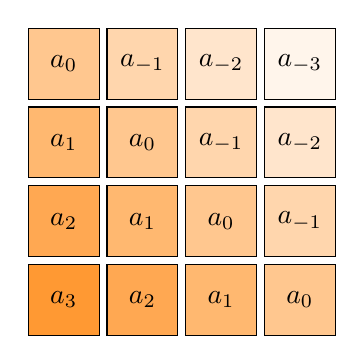
\begin{tikzpicture}
\foreach \i in {0,...,3} {\foreach \j in {0,...,3} {
  \pgfmathtruncatemacro{\d}{\i-\j}
  \pgfmathtruncatemacro{\c}{12*(\d+3)+8}
  \node[draw,minimum size=9mm,inner sep=0,fill=orange!\c] at (\j,-\i) {$a_{\d}$};
}}
\end{tikzpicture}
\caption{Original figure: a $4\times4$ Toeplitz matrix; equal shading = equal entry ($a_{i-j}$).}
\end{figure}

\begin{example}[Convolution as a Toeplitz product]
Let $\mathbf h=(1,2,3)$ and $\mathbf x=(1,0,-1)$. Their full convolution is $\mathbf y=(1,2,2,-2,-3)$, and
\[
\mathbf y=\begin{bmatrix}1&0&0\\2&1&0\\3&2&1\\0&3&2\\0&0&3\end{bmatrix}\begin{bmatrix}1\\0\\-1\end{bmatrix}=\begin{bmatrix}1\\2\\2\\-2\\-3\end{bmatrix}.
\]
\end{example}

\begin{intuition}
A Toeplitz matrix is a weight matrix with a \emph{shared} pattern: the same numbers slide along the diagonals. Convolutional layers are exactly linear layers whose weight matrix is (block-)Toeplitz, which is why they have so few free parameters ($3$ here instead of $5\cdot3=15$).
\end{intuition}

\paragraph{Positive semidefinite matrix \slides{48}.}
\begin{definition}[Positive (semi)definite]
$A\in\K^{N\times N}$ is \emph{positive semidefinite}, $A\succeq0$, if $\Re(\mathbf w\Her A\mathbf w)\ge0$ for all $\mathbf w\in\K^N$; \emph{positive definite}, $A\succ0$, if $\mathbf w\Her A\mathbf w>0$ for all $\mathbf w\ne0$. For two matrices, $A\succeq B$ means $\mathbf z\T A\mathbf z\ge\mathbf z\T B\mathbf z$ for all $\mathbf z$.
\end{definition}

\begin{proposition}\label{prop:gram}
For any $X\in\R^{m\times n}$ the matrix $X\T X$ is positive semidefinite. In particular the covariance matrix of Algorithm~\ref{alg:cov} is.
\end{proposition}
\begin{proof}
$\mathbf w\T X\T X\mathbf w=(X\mathbf w)\T(X\mathbf w)=\|X\mathbf w\|^2\ge0$.
\end{proof}

\begin{example}
$\begin{bmatrix}2&-1\\-1&2\end{bmatrix}$: $\mathbf w\T A\mathbf w=w_1^2+w_2^2+(w_1-w_2)^2>0$ for $\mathbf w\ne0$, so $A\succ0$. $\begin{bmatrix}1&1\\1&1\end{bmatrix}$: $(w_1+w_2)^2\ge0$, zero for $\mathbf w=(1,-1)$: $A\succeq0$ but not $\succ0$. $\begin{bmatrix}1&2\\2&1\end{bmatrix}$: $\mathbf w=(1,-1)$ gives $1-4+1=-2<0$: indefinite.
\end{example}

\begin{figure}[ht]
\centering
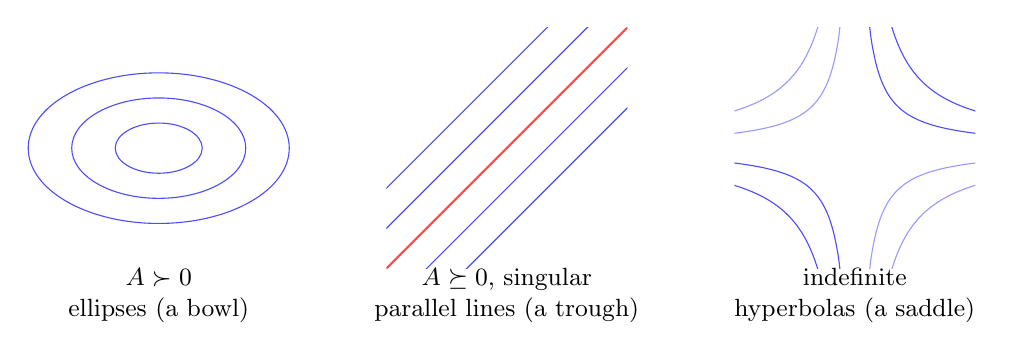
\begin{tikzpicture}[scale=0.85,lab/.style={font=\small,align=center}]
\begin{scope}
  \foreach \r in {0.5,1,1.5} \draw[blue!70] (0,0) ellipse ({1.3*\r} and {0.75*\r});
  \node[lab] at (0,-2.2) {$A\succ0$\\ellipses (a bowl)};
\end{scope}
\begin{scope}[xshift=5.2cm]
  \begin{scope}
  \clip (-1.8,-1.8) rectangle (1.8,1.8);
  \foreach \c in {-1.2,-0.6,0.6,1.2} \draw[blue!70] (-2.4,{-2.4-\c})--(2.4,{2.4-\c});
  \draw[red!70,thick] (-2.4,-2.4)--(2.4,2.4);
  \end{scope}
  \node[lab] at (0,-2.2) {$A\succeq0$, singular\\parallel lines (a trough)};
\end{scope}
\begin{scope}[xshift=10.4cm]
  \begin{scope}
  \clip (-1.8,-1.8) rectangle (1.8,1.8);
  \foreach \c in {0.4,1.0} {
    \draw[blue!70,domain=0.15:2.5,samples=30,smooth,variable=\x] plot ({\x},{\c/\x});
    \draw[blue!70,domain=0.15:2.5,samples=30,smooth,variable=\x] plot ({-\x},{-\c/\x});
    \draw[blue!40,domain=0.15:2.5,samples=30,smooth,variable=\x] plot ({-\x},{\c/\x});
    \draw[blue!40,domain=0.15:2.5,samples=30,smooth,variable=\x] plot ({\x},{-\c/\x});
  }
  \end{scope}
  \node[lab] at (0,-2.2) {indefinite\\hyperbolas (a saddle)};
\end{scope}
\end{tikzpicture}
\caption{Original figure: level sets $\{\mathbf w:\mathbf w\T A\mathbf w=c\}$ for the three cases of the example.}
\end{figure}

\begin{intuition}
$\mathbf w\T A\mathbf w$ asks: ``if I push in direction $\mathbf w$, does the landscape rise?'' Positive definite means rising in every direction (a bowl, a single minimum); semidefinite allows flat directions (a trough); indefinite means some directions go down (a saddle). Covariances, Gram/kernel matrices and, later, Hessians at minima are all of this type.
\end{intuition}

\subsection{Matrix Inversion \slides{49--53}}\label{sec:inv}

\paragraph{Inverse matrix \slides{49--50}.}
\begin{definition}[Inverse]
$A\in(\R,\C)^{N\times N}$ is invertible (nonsingular) if there is $B$ with $BA=I$, where $I=\diag(1,\dots,1)$. Then $B$ is unique, written $A^{-1}$, and $A^{-1}A=I$.
\end{definition}

\begin{theorem}[Inverse of a product; solving $A\mathbf x=\mathbf b$]\label{thm:inv}
If $A,B,C$ are invertible then $(ABC\cdots)^{-1}=\cdots C^{-1}B^{-1}A^{-1}$ and $(A\Her)^{-1}=(A^{-1})\Her$. If $A$ is nonsingular, $A\mathbf x=\mathbf b$ has the unique solution $\mathbf x=A^{-1}\mathbf b$.
\end{theorem}
\begin{proof}
$(AB)(B^{-1}A^{-1})=A(BB^{-1})A^{-1}=AA^{-1}=I$; induction for longer products. Taking $\Her$ of $AA^{-1}=I$ and using Proposition~\ref{prop:transp} gives $(A^{-1})\Her A\Her=I$. Existence: $A(A^{-1}\mathbf b)=\mathbf b$. Uniqueness: $A\mathbf x=\mathbf b\Rightarrow\mathbf x=A^{-1}A\mathbf x=A^{-1}\mathbf b$.
\end{proof}

\begin{remark}
The definition asks only for $BA=I$; for \emph{square} matrices this implies $AB=I$ (a left inverse forces $A$ to be injective, hence bijective in finite dimension), which justifies calling $B$ ``the'' inverse. The slide's list also contains $(A+B)\Her=A\Her+B\Her$ and $(AB)\Her=B\Her A\Her$; these are transpose rules (Proposition~\ref{prop:transp}), not inverse rules.
\end{remark}

\begin{intuition}
Inverting a product reverses the order too, for the same reason as transposing: to undo ``put on socks, then shoes'' you first remove the shoes. And $A^{-1}$ is ``the undo button'' of the linear map $A$: it exists only if $A$ loses no information.
\end{intuition}

\paragraph{Pseudoinverse matrix \slides{51--52}.}
\begin{definition}[Moore--Penrose pseudoinverse]
For a general (rectangular) $A\in(\R,\C)^{N\times M}$, the pseudoinverse $A\pinv\in(\R,\C)^{M\times N}$ is the matrix satisfying
\[
AA\pinv A=A,\qquad A\pinv AA\pinv=A\pinv,\qquad (AA\pinv)\Her=AA\pinv,\qquad (A\pinv A)\Her=A\pinv A .
\]
\end{definition}

\begin{proposition}[Uniqueness]\label{prop:pinv-unique}
There is at most one matrix satisfying the four conditions.
\end{proposition}
\begin{proof}
Let $X,Y$ both satisfy them. Then $AX=(AYA)X=AY(AX)=(AY)\Her(AX)\Her=(AXAY)\Her=(AY)\Her=AY$, and likewise $XA=X(AYA)=(XA)(YA)=(XA)\Her(YA)\Her=(YAXA)\Her=(YA)\Her=YA$. Hence $X=XAX=X(AX)=X(AY)=(XA)Y=(YA)Y=Y$.
\end{proof}

\begin{theorem}[Full-rank formulas \slides{52}]\label{thm:pinv}
Assume $A$ has full rank. Then
\[
A\pinv=\begin{cases}A^{-1}&N=M\ (\text{square}),\\ A\Her(AA\Her)^{-1}&N<M\ (\text{``fat''}),\\ (A\Her A)^{-1}A\Her&N>M\ (\text{``tall''}).\end{cases}
\]
In all three cases, if $A\mathbf x=\mathbf b$ is consistent, $\mathbf x=A\pinv\mathbf b$ is a solution.
\end{theorem}
\begin{proof}
Tall case. Full column rank makes $A\Her A$ invertible: $A\Her A\mathbf x=0\Rightarrow\|A\mathbf x\|^2=\mathbf x\Her A\Her A\mathbf x=0\Rightarrow A\mathbf x=0\Rightarrow\mathbf x=0$. Put $A\pinv=(A\Her A)^{-1}A\Her$. Then $A\pinv A=I$ (Hermitian) gives conditions 2 and 4 immediately (condition 2: $A\pinv AA\pinv=A\pinv$), condition 1: $AA\pinv A=A$, and $AA\pinv=A(A\Her A)^{-1}A\Her$ is Hermitian. The fat case is the same computation with $A\Her$ in place of $A$ and $AA\Her$ invertible (full row rank); the square case is the ordinary inverse. Finally, if $A\mathbf x_0=\mathbf b$, then $AA\pinv\mathbf b=AA\pinv A\mathbf x_0=A\mathbf x_0=\mathbf b$.
\end{proof}

\begin{figure}[ht]
\centering
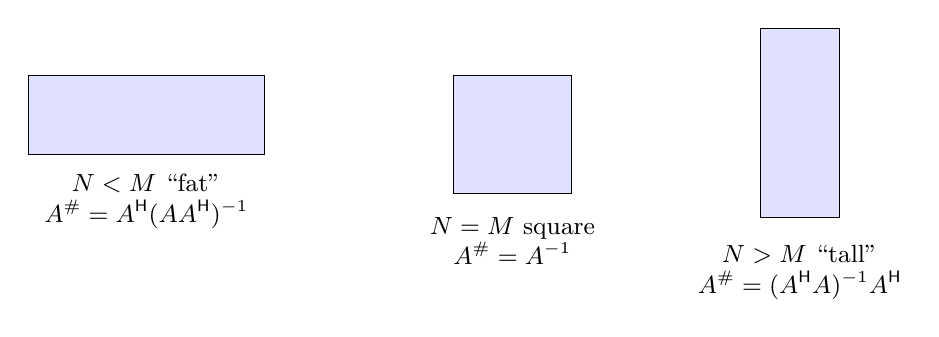
\begin{tikzpicture}[lab/.style={font=\small,align=center}]
\draw[fill=blue!12] (0,0) rectangle (3,1.0);
\node[lab] at (1.5,-0.6) {$N<M$ ``fat''\\$A\pinv=A\Her(AA\Her)^{-1}$};
\draw[fill=blue!12] (5.4,-0.5) rectangle (6.9,1.0) ;
\node[lab] at (6.15,-1.1) {$N=M$ square\\$A\pinv=A^{-1}$};
\draw[fill=blue!12] (9.3,-0.8) rectangle (10.3,1.6);
\node[lab] at (9.8,-1.5) {$N>M$ ``tall''\\$A\pinv=(A\Her A)^{-1}A\Her$};
\end{tikzpicture}
\caption{Original figure: the three shapes of $A$ and the matching full-rank formulas.}
\end{figure}

\begin{algorithm}[Solving $A\mathbf x=\mathbf b$ with the pseudoinverse]
(1) Read off $N,M$ from the shape of $A$ and check that $A$ has full rank. (2) Pick the formula for $A\pinv$ from Theorem~\ref{thm:pinv} (other methods compute $A\pinv$ via matrix decompositions). (3) Return $\mathbf x=A\pinv\mathbf b$.
\end{algorithm}

\begin{intuition}
An ordinary inverse needs a square, lossless matrix. The pseudoinverse is the best available substitute for the rest: a tall matrix has more equations than unknowns (overdetermined; $A\pinv$ is the \emph{left} inverse, $A\pinv A=I$), a fat one has more unknowns than equations (underdetermined; $A\pinv$ is a \emph{right} inverse, $AA\pinv=I$). Example: for the tall $A=\begin{bmatrix}1\\1\end{bmatrix}$, $A\pinv=\tfrac12\begin{bmatrix}1&1\end{bmatrix}$, so $A\pinv\mathbf b$ is the \emph{average} of the two equations' right-hand sides. Note that the slide's formulas assume full rank; the general definition (four conditions) does not.
\end{intuition}

\paragraph{Matrix inversion lemma \slides{53}.}
\begin{theorem}[Matrix inversion lemma]\label{thm:mil}
Let $A\in\K^{M\times M}$, $B\in\K^{M\times N}$, $C\in\K^{N\times N}$, $D\in\K^{N\times M}$, with $A$, $C$ and $S=C^{-1}+DA^{-1}B$ invertible. Then
\[
[A+BCD]^{-1}=A^{-1}-A^{-1}B\big(C^{-1}+DA^{-1}B\big)^{-1}DA^{-1}.
\]
\end{theorem}
\begin{proof}
Multiply the left factor by the claimed right-hand side:
$(A+BCD)\big(A^{-1}-A^{-1}BS^{-1}DA^{-1}\big)=I+B\big[C-S^{-1}-CDA^{-1}BS^{-1}\big]DA^{-1}$.
Since $C=CSS^{-1}=C(C^{-1}+DA^{-1}B)S^{-1}=S^{-1}+CDA^{-1}BS^{-1}$, the bracket vanishes and the product is $I$.
\end{proof}

\begin{corollary}[Rank-one update, Sherman--Morrison]
For $C=1$, $B=\mathbf u$, $D=\mathbf v\Her$: $(A+\mathbf u\mathbf v\Her)^{-1}=A^{-1}-\dfrac{A^{-1}\mathbf u\mathbf v\Her A^{-1}}{1+\mathbf v\Her A^{-1}\mathbf u}$.
\end{corollary}

\begin{example}
$A=2I_2$, $\mathbf u=\mathbf v=[1,1]\T$: $A+\mathbf u\mathbf v\T=\begin{bmatrix}3&1\\1&3\end{bmatrix}$. Formula: $A^{-1}=\tfrac12I$, $\mathbf v\T A^{-1}\mathbf u=1$, so the inverse is $\tfrac12I-\tfrac{1}{2}\cdot\tfrac14\begin{bmatrix}1&1\\1&1\end{bmatrix}=\tfrac18\begin{bmatrix}3&-1\\-1&3\end{bmatrix}$, which indeed multiplies $\begin{bmatrix}3&1\\1&3\end{bmatrix}$ to $I$.
\end{example}

\begin{intuition}
In online learning a matrix is updated by a small change every time a new sample arrives. Re-inverting an $M\times M$ matrix from scratch costs $O(M^3)$; the lemma says that if the update has low rank $N\ll M$, the new inverse is the old one plus a correction that only requires inverting an $N\times N$ matrix. This is why it is ``a very useful property in the development of online machine learning algorithms''.
\end{intuition}

\subsection{Rank and Determinant of a Matrix \slides{54}}

\begin{definition}[Rank, determinant]
The rank $r=\rank(A)$ of $A\in\R^{M\times N}$ is the number of linearly independent columns. The determinant of a square matrix, $\det(A)$ or $\Delta_A$, can be computed by several algorithms depending on size.
\end{definition}

\begin{theorem}[Solvability of linear systems]\label{thm:rc}
$A\mathbf x=\mathbf b$ admits a solution iff $\rank(A)=\rank([A\ \mathbf b])$, i.e.\ the rank of the coefficient matrix equals the rank of the complete matrix. For square $A$: $A$ is invertible $\iff\rank(A)=N\iff\det(A)\ne0$.
\end{theorem}
\begin{proof}[Proof sketch]
$A\mathbf x=\mathbf b$ is solvable iff $\mathbf b$ is a linear combination of the columns of $A$, i.e.\ iff appending $\mathbf b$ does not enlarge the column space, iff the two ranks agree. The square-matrix equivalences are the standard characterizations of invertibility (full rank means the columns form a basis; $\det\neq0$ is the algebraic test for this).
\end{proof}

\begin{intuition}
Rank is the number of \emph{genuinely different} directions a matrix produces. Example: $\begin{bmatrix}1&2\\2&4\end{bmatrix}$ has rank 1 (second column $=2\times$ first), $\det=1\cdot4-2\cdot2=0$: it squashes the plane onto a line, information is lost, no inverse exists, and $A\mathbf x=\mathbf b$ is solvable only if $\mathbf b$ lies on that line. This is the bridge to the pseudoinverse (what to do when there is no ordinary inverse) and, in the sections not covered here, to the SVD.
\end{intuition}

%====================================================================
\section*{Appendix A: Supplementary material \emph{(not on the slides)}}\label{app:supp}
\addcontentsline{toc}{section}{Appendix A: Supplementary material (not on the slides)}
%====================================================================

\begin{tcolorbox}[colback=yellow!8,colframe=yellow!50!black,boxrule=0.5pt,arc=2pt]
\small The items below are \textbf{not} part of the slides (1--54). They support material that the slides mention and are included for completeness; they are my own standard derivations, since no companion chapter was provided.
\end{tcolorbox}

\begin{proposition}[Mixed product of Kronecker products; supplements slide 37]
$(A\otimes B)(C\otimes D)=(AC)\otimes(BD)$ whenever the products $AC$ and $BD$ are defined.
\end{proposition}
\begin{proof}
The $(i,j)$ block of $(A\otimes B)(C\otimes D)$ is $\sum_k(a_{ik}B)(c_{kj}D)=\big(\sum_ka_{ik}c_{kj}\big)BD=(AC)_{ij}BD$, which is the $(i,j)$ block of $(AC)\otimes(BD)$.
\end{proof}

\begin{proposition}[$\vecop$ and Kronecker product; links slides 37 and 42]
For compatible $A,X,B$: $\vecop(AXB)=(B\T\otimes A)\vecop(X)$.
\end{proposition}
\begin{proof}
Let $\mathbf x_k$ be the columns of $X$ and $\mathbf b_j$ the columns of $B$. The $j$-th column of $AXB$ is $A X\mathbf b_j=A\sum_k b_{kj}\mathbf x_k=\sum_k b_{kj}A\mathbf x_k$. The $j$-th block row of $B\T\otimes A$ has blocks $(B\T)_{jk}A=b_{kj}A$, so multiplying by $\vecop(X)=[\mathbf x_1;\dots;\mathbf x_K]$ gives exactly that sum.
\end{proof}

\begin{intuition}
A linear map that acts on the \emph{columns} of $X$ by $A$ and on its \emph{rows} by $B$ is, once $X$ is flattened with $\vecop$, a single (huge) matrix $B\T\otimes A$. The slide's remark about the tensor product of linear maps is exactly this statement. In practice one never forms the Kronecker matrix: one computes $AXB$, which is far cheaper.
\end{intuition}

\begin{proposition}[Equivalent tests for positive semidefiniteness; supplements slide 48]
For real symmetric $A$: $A\succeq0\iff$ all eigenvalues are $\ge0\iff A=M\T M$ for some $M$.
\end{proposition}
\begin{proof}
Write $A=Q\Lambda Q\T$ (spectral theorem, $Q$ orthogonal). Then $\mathbf w\T A\mathbf w=\sum_i\lambda_i(Q\T\mathbf w)_i^2$, which is $\ge0$ for all $\mathbf w$ iff every $\lambda_i\ge0$ (choose $\mathbf w=Q\mathbf e_i$). If $\lambda_i\ge0$, take $M=\Lambda^{1/2}Q\T$; conversely $A=M\T M$ is PSD by Proposition~\ref{prop:gram}.
\end{proof}

\begin{proposition}[Pseudoinverse via SVD; anticipates later lectures]
If $A=U\Sigma V\T$ is a (compact) SVD with positive singular values, then $A\pinv=V\Sigma^{-1}U\T$.
\end{proposition}
\begin{proof}
With $U\T U=V\T V=I$: $AA\pinv A=U\Sigma V\T V\Sigma^{-1}U\T U\Sigma V\T=U\Sigma V\T=A$; $A\pinv AA\pinv=A\pinv$ likewise; $AA\pinv=UU\T$ and $A\pinv A=VV\T$ are symmetric. By Proposition~\ref{prop:pinv-unique} this is \emph{the} pseudoinverse.
\end{proof}

\begin{intuition}
The SVD writes any matrix as ``rotate, scale each axis, rotate''. The pseudoinverse simply undoes each nonzero scaling and ignores the directions that were squashed to zero --- the ones that carried no information and therefore cannot be recovered.
\end{intuition}

%====================================================================
\section{Summary}
%====================================================================

\subsection{Comparison of the operations covered}

\begin{center}
\footnotesize
\renewcommand{\arraystretch}{1.25}
\begin{tabular}{@{}p{2.6cm}p{2.5cm}p{3.1cm}p{2.3cm}p{3.6cm}@{}}
\toprule
Operation & Notation & Shapes & Sums over an index? & Role in neural networks\\\midrule
Dot product & $\mathbf u\T\mathbf v$ & $N,N\to$ scalar & yes, all & weighted sum in a neuron; similarity\\
Outer product & $\mathbf u\mathbf v\T$ & $M,N\to M\times N$ & no & rank-one matrices; gradient of a linear layer\\
Matrix product & $AB$ & $(N\times P)(P\times M)\to N\times M$ & yes, shared axis $P$ & linear layer $XW$; attention scores\\
Hadamard & $A\Had B$ & equal shapes & no & gates, masks, ReLU derivative\\
Kronecker & $A\otimes B$ & $(P\times Q),(N\times M)\to PN\times QM$ & no & tensor product of maps\\
Transpose / $\Her$ & $A\T$, $A\Her$ & $N\times M\to M\times N$ & --- & reverses products; backward pass\\
$\vecop$ / reshape & $\vecop(A)$ & $N\times M\to NM\times1$ & --- & flattening, heads, patches\\
Inverse & $A^{-1}$ & square, full rank & --- & solving $A\mathbf x=\mathbf b$; undo a lossless map\\
Pseudoinverse & $A\pinv$ & any $N\times M$ & --- & least-squares/underdetermined systems\\
Inversion lemma & $[A+BCD]^{-1}$ & $M\times M$, low-rank update & --- & online algorithms\\\bottomrule
\end{tabular}
\end{center}

\begin{center}
\footnotesize
\begin{tabular}{@{}lll@{}}
\toprule
Special matrix & Defining property & Example of where it appears\\\midrule
Diagonal & $a_{ij}=0$, $i\ne j$ & per-feature scaling ($D_{\mathbf a}\mathbf x=\mathbf a\Had\mathbf x$)\\
Symmetric / Hermitian & $A\T=A$ / $A\Her=A$ & covariance, kernels\\
Toeplitz & $a_{ij}=a_{i-j}$ & convolution as matrix product\\
Positive (semi)definite & $\mathbf w\Her A\mathbf w>0$ ($\ge0$) & covariance, Gram matrices, Hessians at minima\\\bottomrule
\end{tabular}
\end{center}

\subsection{Cost of the three ``products''}

\begin{figure}[ht]
\centering
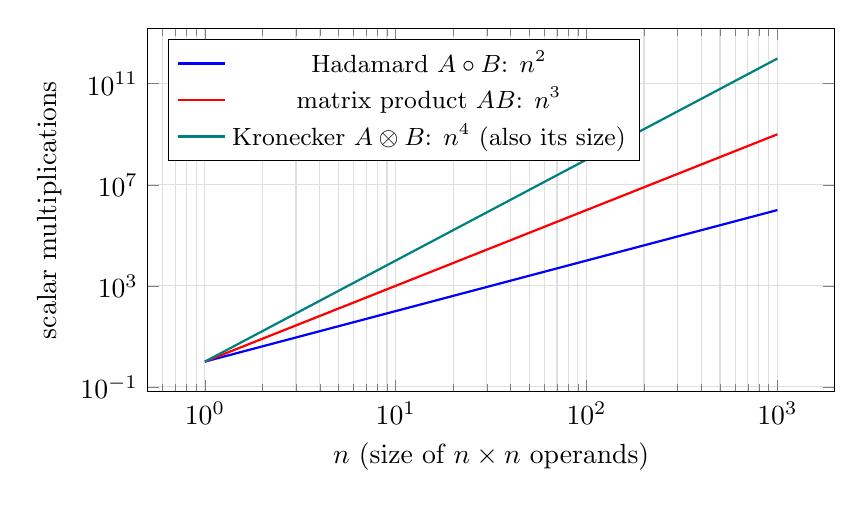
\begin{tikzpicture}
\begin{loglogaxis}[width=0.85\linewidth,height=6.2cm,xlabel={$n$ (size of $n\times n$ operands)},
  ylabel={scalar multiplications},legend pos=north west,legend style={font=\small},grid=both,
  grid style={gray!25}]
\addplot[thick,blue,domain=1:1000,samples=20] {x^2}; \addlegendentry{Hadamard $A\Had B$: $n^2$}
\addplot[thick,red,domain=1:1000,samples=20] {x^3}; \addlegendentry{matrix product $AB$: $n^3$}
\addplot[thick,teal,domain=1:1000,samples=20] {x^4}; \addlegendentry{Kronecker $A\otimes B$: $n^4$ (also its size)}
\end{loglogaxis}
\end{tikzpicture}
\caption{Original qualitative comparison: the Hadamard product touches each entry once, the matrix product mixes rows with columns, and the Kronecker product produces an $n^2\times n^2$ matrix --- which is why it is used conceptually rather than materialized.}
\end{figure}

\subsection{Key take-aways}
\begin{enumerate}
  \item One forward--backward step is read through three lenses (linear algebra, geometry, optimization), and one must not confuse \emph{representation space} (activations) with \emph{parameter space} (models).
  \item Without nonlinearity a stack of affine layers collapses to one affine map (Proposition~\ref{prop:collapse}); depth only matters because of $\sigma$.
  \item Tensors get their meaning from the \emph{labels of their axes}; matrix products are \emph{contractions} of a shared axis, and checking shapes before coding catches most errors.
  \item Matrix product mixes information across features, whereas the Hadamard product gates entries individually; the ReLU derivative is a Hadamard mask.
  \item When $A$ is not square and invertible, the pseudoinverse provides $\mathbf x=A\pinv\mathbf b$; low-rank updates are handled efficiently by the matrix inversion lemma, and rank/determinant tell whether an inverse or a solution exists.
\end{enumerate}

\end{document}